% \documentclass[handout]{beamer}
\documentclass{beamer}

\usetheme{Copenhagen}

\usepackage{amsbsy}
% \usepackage{amsmath}
\usepackage{amstext}
\usepackage{amsfonts}
\usepackage{amssymb}
\usepackage{amsthm}
\usepackage{shadow}% kotak shadow
\usepackage{biblatex}

\newcommand{\R}{\mathbb{R}}
\newcommand{\E}{\mathbb{E}}
\newcommand{\RCH}{\text{RCH}}
\newcommand{\CH}{\text{CH}}
\newcommand{\Prob}{\mathbb{P}}
\newcommand{\F}{\mathcal{F}}
\newcommand{\G}{\mathcal{G}}
\newcommand{\B}{\mathcal{B}}
\newtheorem*{prop}{Proposition}
\newtheorem*{prob}{Problem}
\newcommand{\rch}{\operatorname{RCH}}

\usepackage{tikz}

\usepackage{curves}
\usepackage{graphics}
\usepackage{graphicx}
\usepackage{color}%masukan colorbegi
\usepackage{makeidx}
\makeindex

%\setbeamertemplate{footline}{}
\setbeamertemplate{footline}[frame number]
\title[Double Descent Demystified]{Double Descent Demystified: Identifying, Interpreting \& Ablating the Sources of a Deep Learning Puzzle}
\subtitle[Rylan Schaeffer, ]{Rylan Schaeffer, Mikail Khona, Zachary Robertson, Akhilan Boopathy, Kateryna Pistunova, Jason W. Rocks, Ila Rani Fiete, and Oluwasanmi Koyejo}
\author{A review by Jack Hanke}

\usepackage{graphicx}
\usepackage{eso-pic}

\newcommand\BackgroundPic{%
\put(0,0){%
\parbox[b][\paperheight]{\paperwidth}{%
\vfill
\centering
\includegraphics[width=\paperwidth,height=\paperheight,%
keepaspectratio]{sfondo.png}%
}}}

% \author[Hanke]{Jack Hanke}
\vfill
% \date{2024}

\subject{fjj}

\AtBeginSection{
\begin{frame}{Outline}
    \tableofcontents[currentsection]
\end{frame}
}
    
\begin{document}

\usetikzlibrary{calc}

\setbeamertemplate{caption}{\raggedright\insertcaption\par}
\usebackgroundtemplate{}


\begin{frame}
    \titlepage
\end{frame}


\begin{frame}{Setting the scene...}
    It's 2001, and Alex Krizhevsky, Ilya Sutskever, and Geoffrey Hinton want to win the ImageNet LSVRC-2010 contest, an image classification competition with over $1000$ different classes of images. 
    
    \begin{center}
        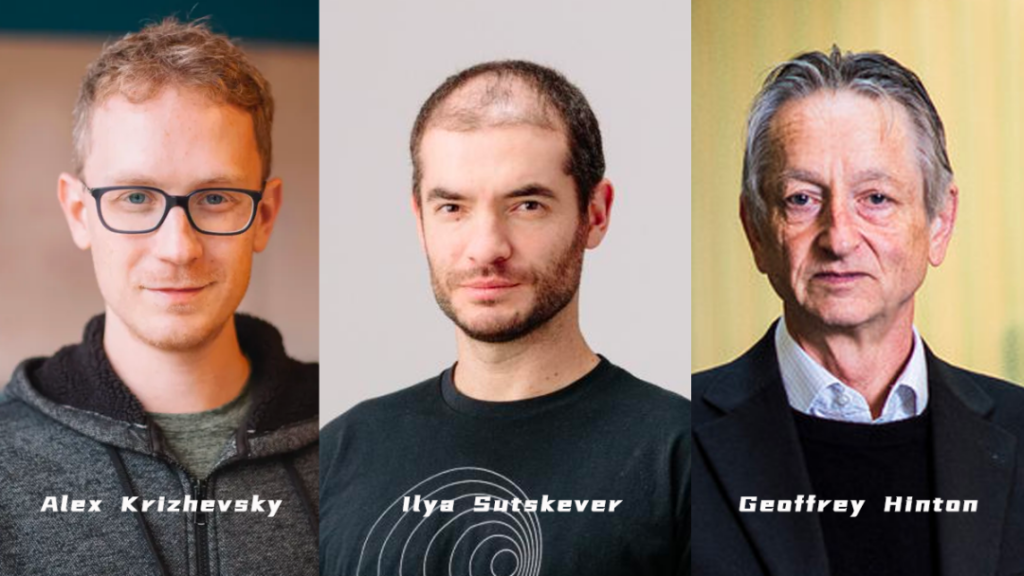
\includegraphics[scale=0.25]{theboys.png}    
    \end{center}

\end{frame}


\begin{frame}{Setting the scene...}
    
    They use a subset of the ImageNet dataset consisting of $1.2$ Million $256 \times 256$ images to train a $60$ million parameter convolutional neural network they called \emph{AlexNet}.

    \begin{center}
        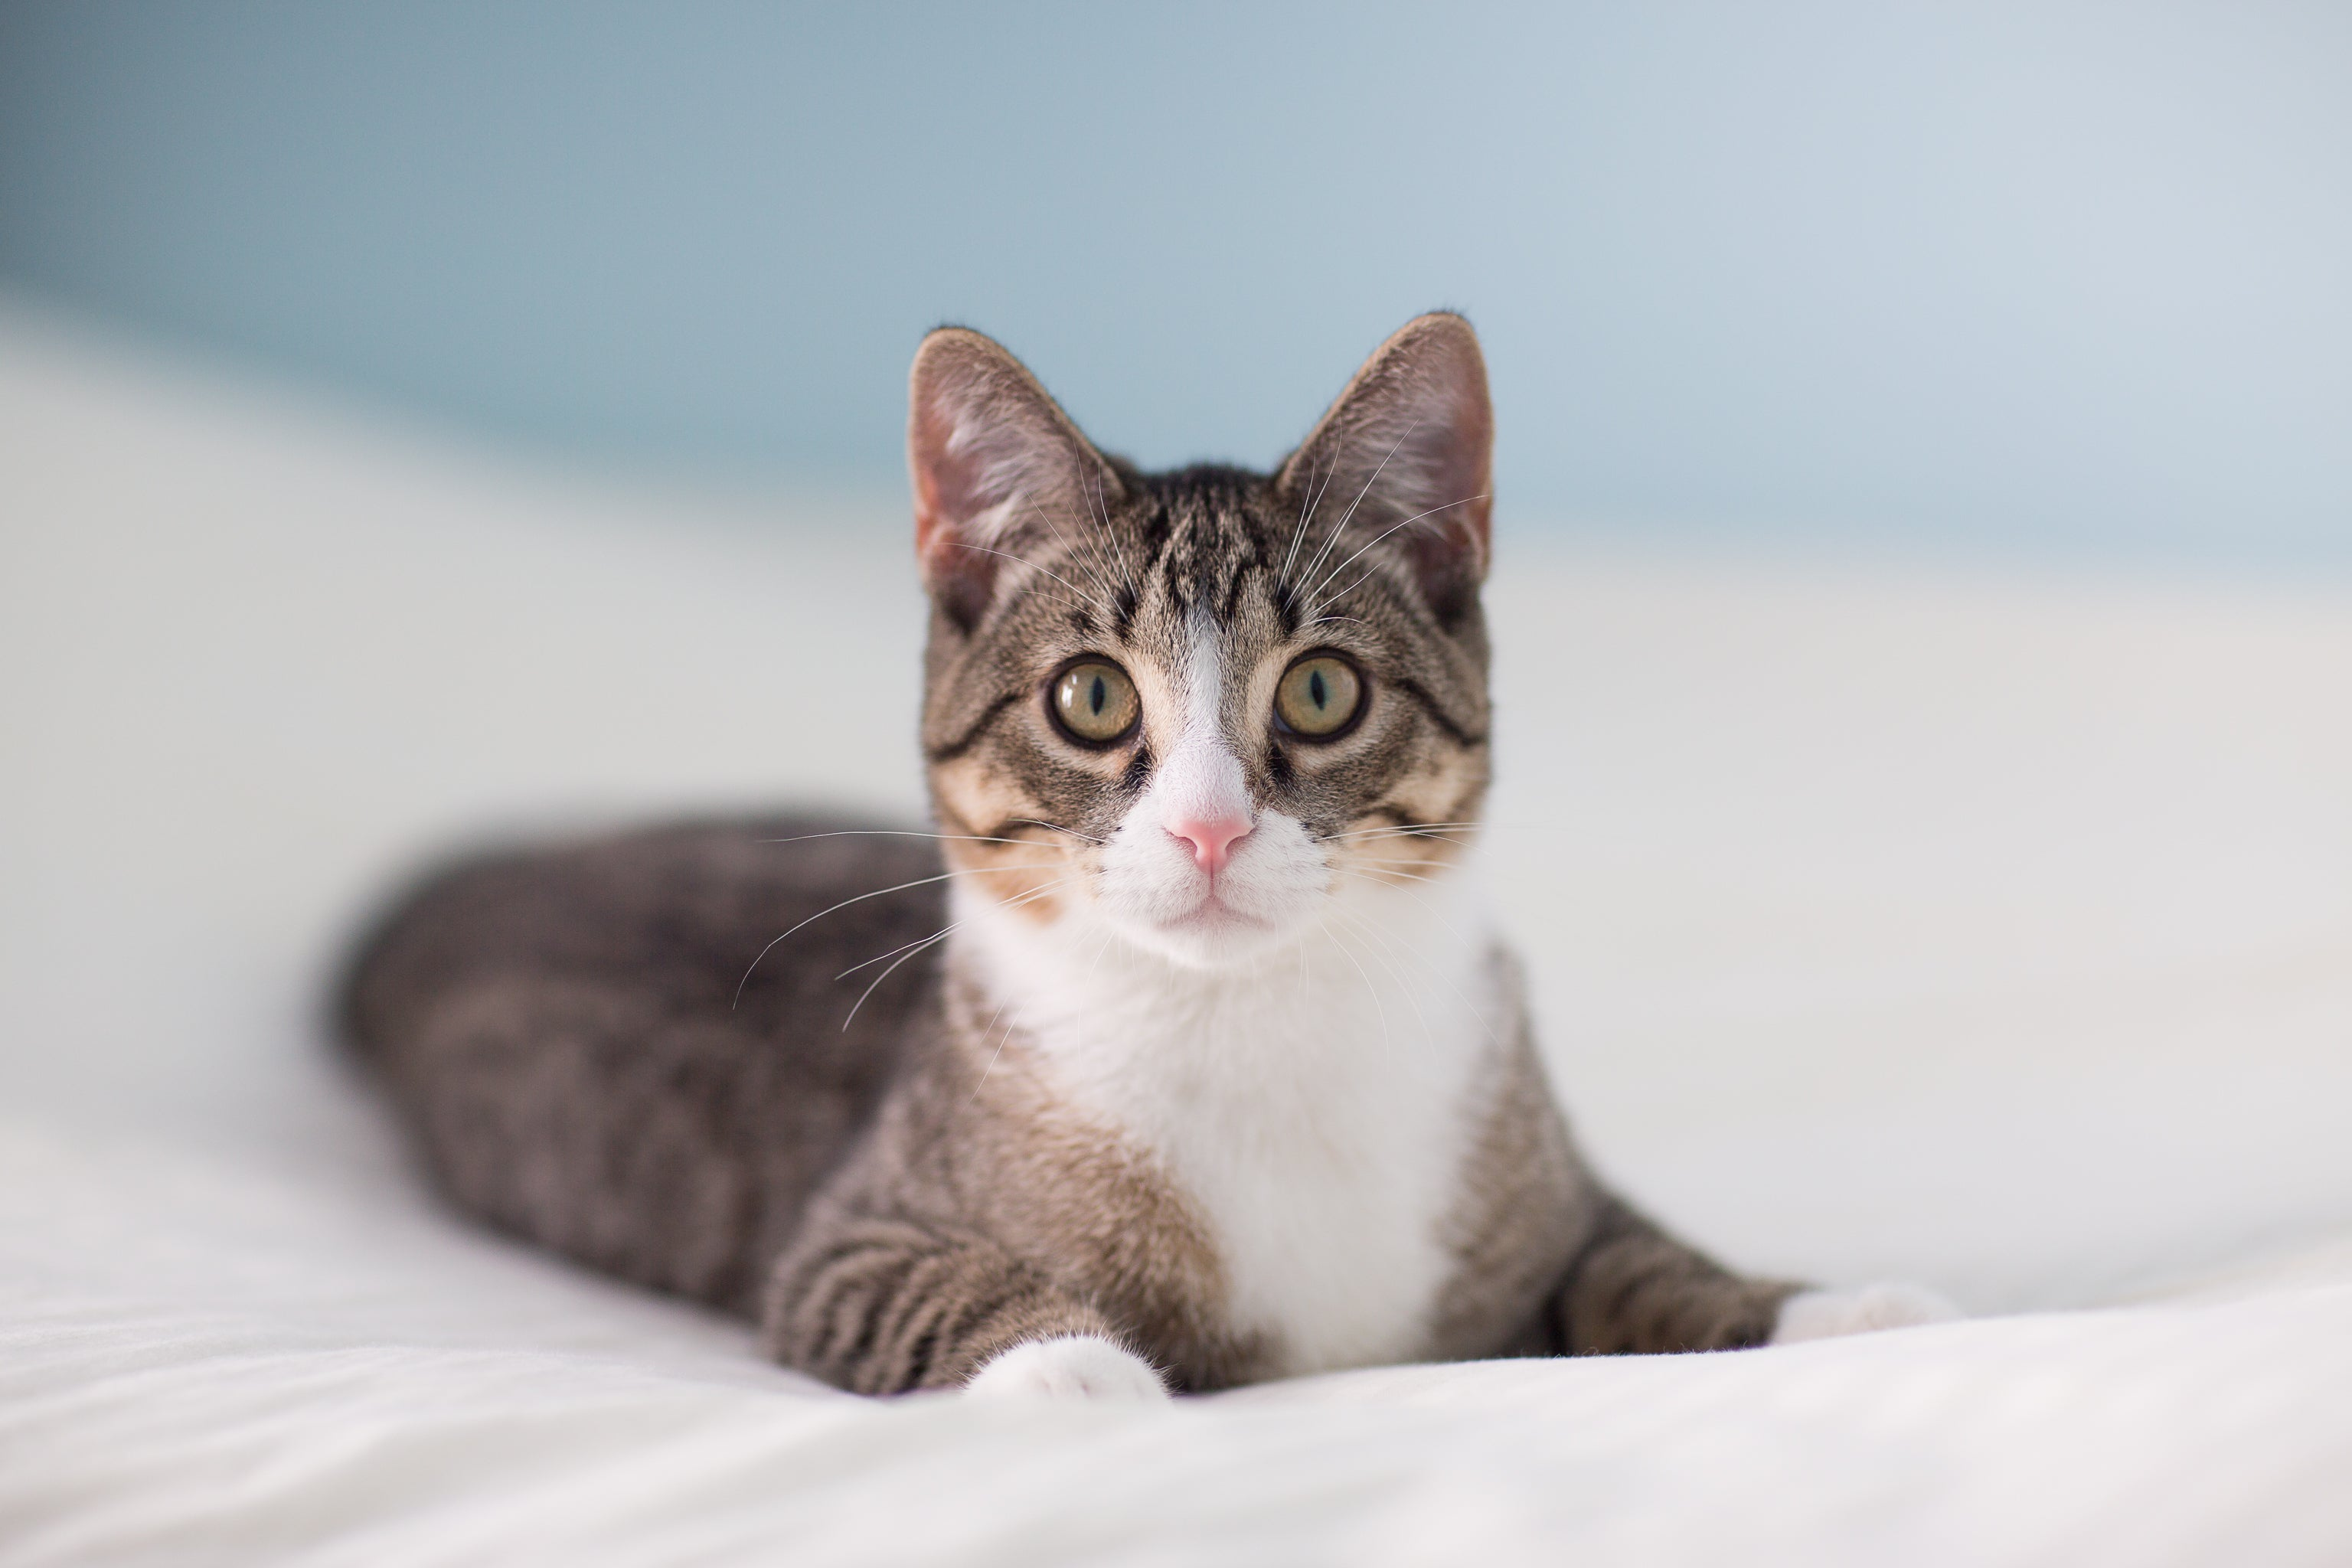
\includegraphics[scale=0.03]{imagenetcat.jpg}    
    \end{center}

    \pause
    
    Alexnet achieves state-of-the-art performance and propels the study of deep learning into the mainstream. 

    \hspace{3cm}
    \pause
    
    Likely indirectly due to their work, we have all been in a similar situation. You solved a problem with a neural network and now have a large collection of inscrutable weights $\theta$.
     
\end{frame}

\begin{frame}{Congrats! You just trained a model!}
\pause
\begin{center}
\begin{enumerate}
\item[Question:] How does your model work?
\pause
\begin{itemize}
    \item What does $\theta_{343}$ do in service of the final output? This is the \emph{blackbox problem}.
    \pause
    \item The answer to this is the world of interpretability research, and is dependent on the specific problem your model is trying to solve. 
    \pause
\end{itemize}
\item[Question:] Why does your model work?
\pause
\begin{itemize}
    \item Why does a model with so many parameters not just memorize the data? This is the \emph{double descent problem}.
    \pause
    \item The answer to this is (in part) this paper. 
\end{itemize}
\end{enumerate}
\end{center}

\end{frame}


\begin{frame}{The Traditional View}
    \begin{center}
        \begin{minipage}{0.45\textwidth}
            \centering
            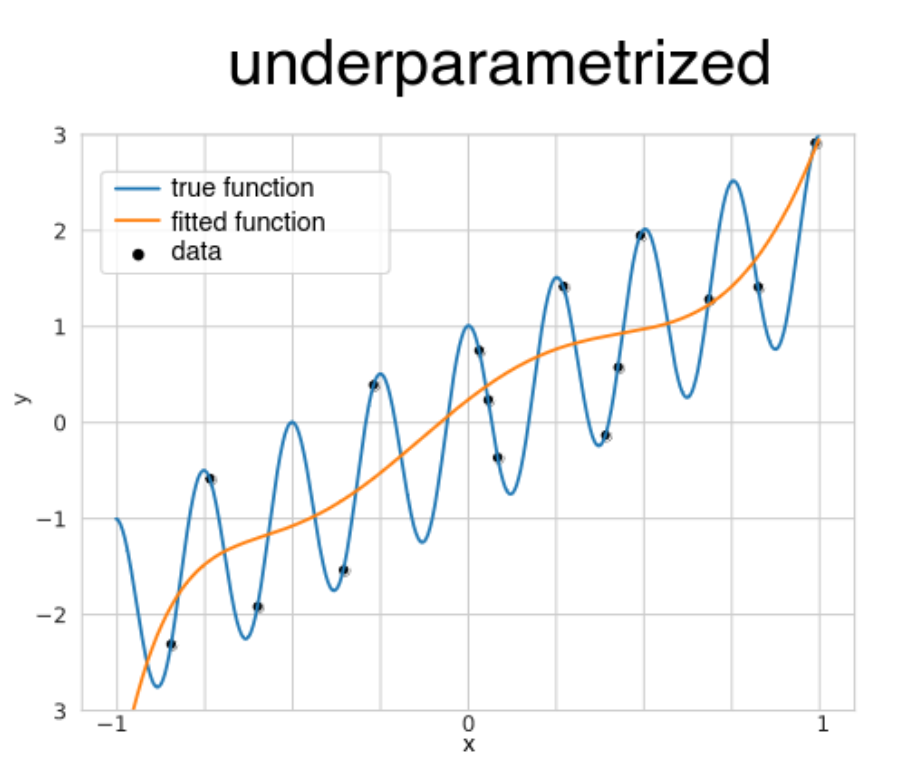
\includegraphics[scale=0.18]{underparam.png}
        \end{minipage}\hfill
        \begin{minipage}{0.45\textwidth}
            \centering
            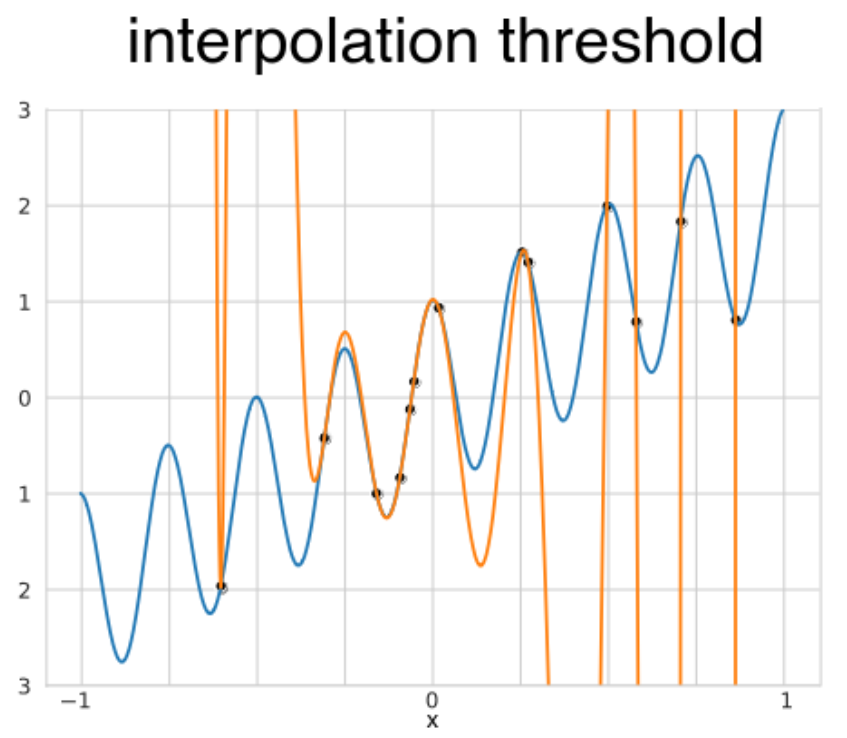
\includegraphics[scale=0.18]{interpolationth.png}
        \end{minipage}
    \end{center}
\end{frame}


\begin{frame}{What (often) actually happens}
\begin{center}
    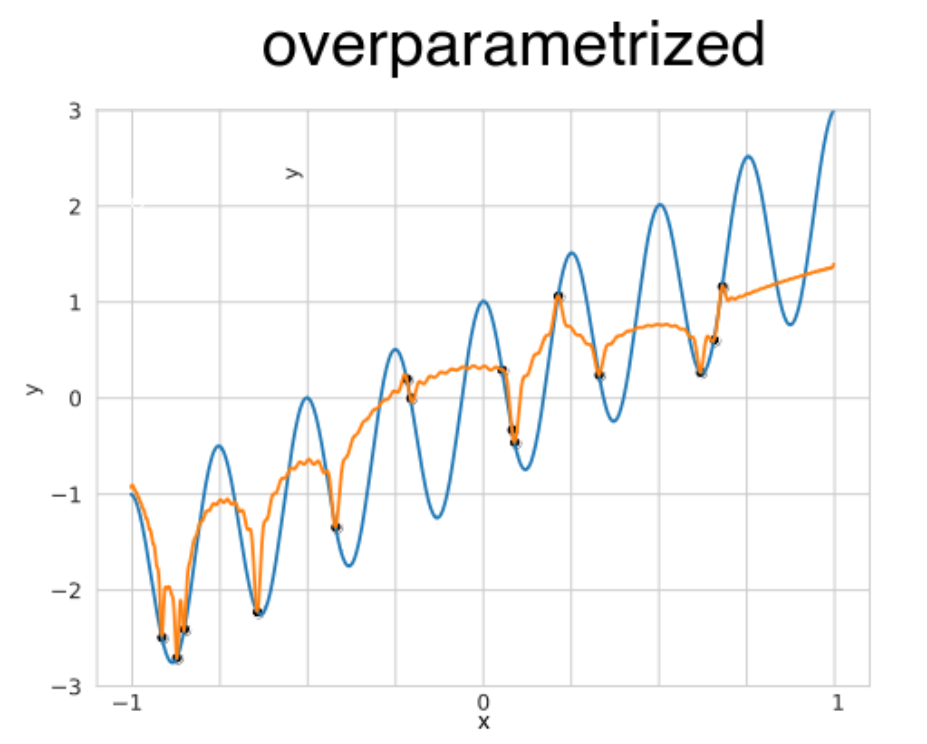
\includegraphics[scale=0.28]{overparam.png}
\end{center}

\end{frame}


\begin{frame}{What is double descent?}
    
This paper defines \href{https://www.youtube.com/watch?v=Kih-VPHL3gA}{double descent} as: \\
\hspace{1.5cm}

\emph{A phenomenon in machine learning that many classes of models can, under relatively broad conditions, exhibit where as the number of parameters increases, the test loss falls, rises, then falls again.}
\pause
\begin{center}
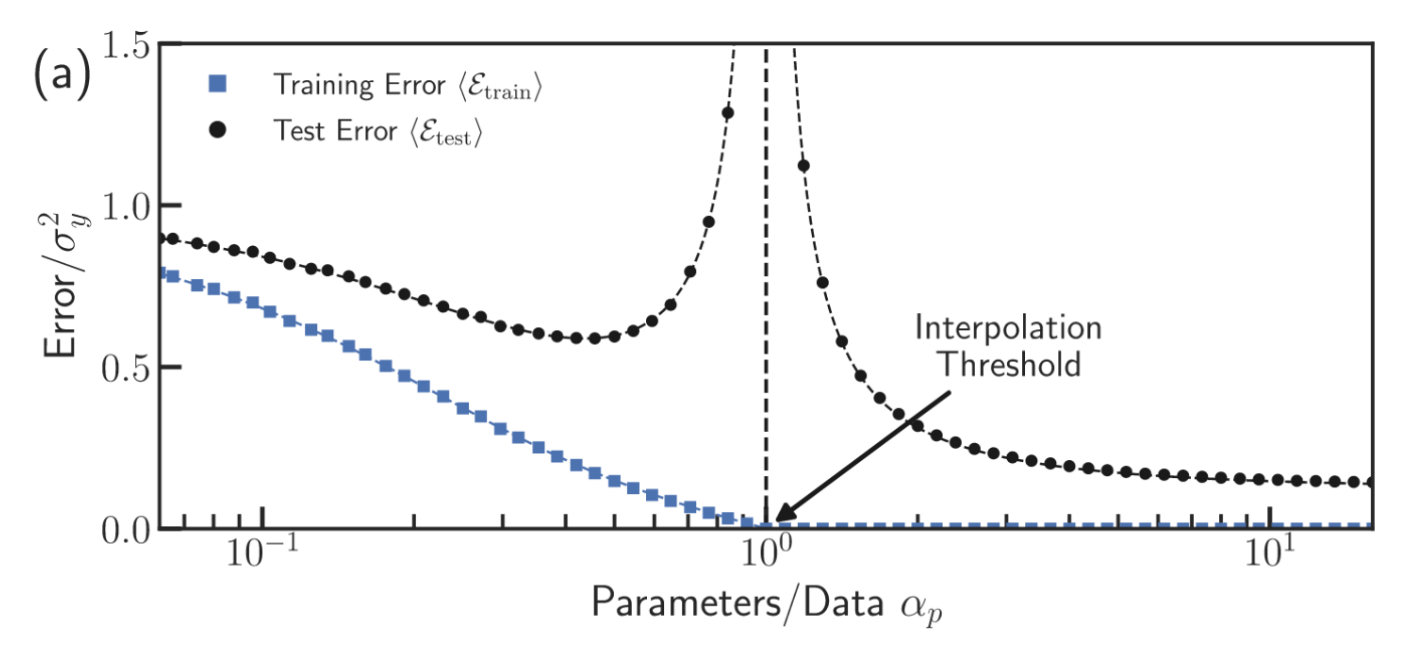
\includegraphics[scale=0.22]{ddd.png}
\end{center}

\end{frame}


\begin{frame}{Double descent in polynomial regression}
\begin{center}
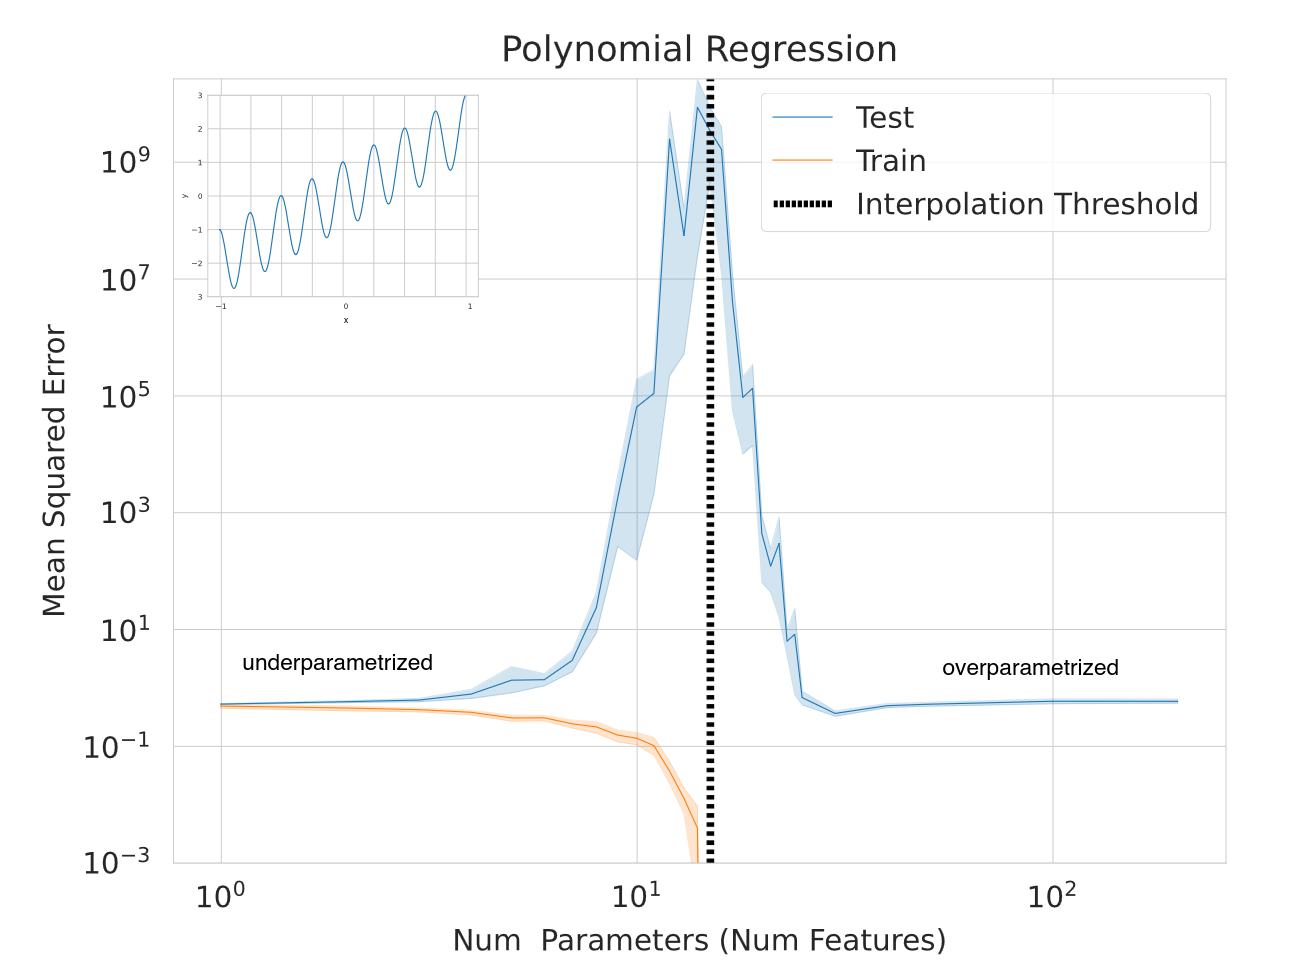
\includegraphics[scale=0.22]{polyreg.png}
\end{center}
\end{frame}


\begin{frame}{Terminology}
    \begin{itemize}
        \item Let $P$ be the number of models parameters
        \item Let $N$ be the number of training data
        \item Let $D$ be the dimensionality of the data
    \end{itemize}
    
    \pause
    
    \begin{itemize}
        \item A model is \emph{underparameterized} if $\frac{N}{P} > 1$
        \item A model is \emph{overparameterized} if $\frac{N}{P} < 1$
        \item A model is at the \emph{interpolation threshold} if $\frac{N}{P} = 1$
    \end{itemize}
    
    \pause
    \hspace{5cm}

    We will next study linear models, which have a fixed value of $P=D+1$. Therefore, double descent occurs in the direction of increasing $N$.

\end{frame}


\begin{frame}{Double descent in linear regression}

    The underparametrized regime is the classic least-squares minimization problem:

    $$\hat{\vec{\beta}}_{under} = \text{arg} \text{min}_{\vec{\beta}}||X \vec{\beta} - Y||^2_2, $$

    which is solved by

    $$\vec{\beta}_{under} = (X^T X)^{-1} X^T Y.$$

    \pause

    For the overparameterized regime, the above optimization problem has infinite solutions. Therefore, we need to choose a different optimization problem:

    $$\hat{\vec{\beta}}_{over} = \text{arg} \text{min}_{\vec{\beta}}||\vec{\beta}||^2_2 \text{   s.t.   } \forall n \in (1,\dots,N) \text{   } \vec{x}_n \vec{\beta} = y_n$$

    which is solved by

    $$\vec{\beta}_{over} = X^T (X X^T)^{-1}Y.$$

\end{frame}


\begin{frame}{Why this choice?}
    $$\hat{\vec{\beta}}_{over} = \text{arg} \text{min}_{\vec{\beta}}||\vec{\beta}||^2_2 \text{   s.t.   } \forall n \in (1,\dots,N) \text{   } \vec{x}_n \vec{\beta} = y_n$$

    \pause
    
    \begin{center}
        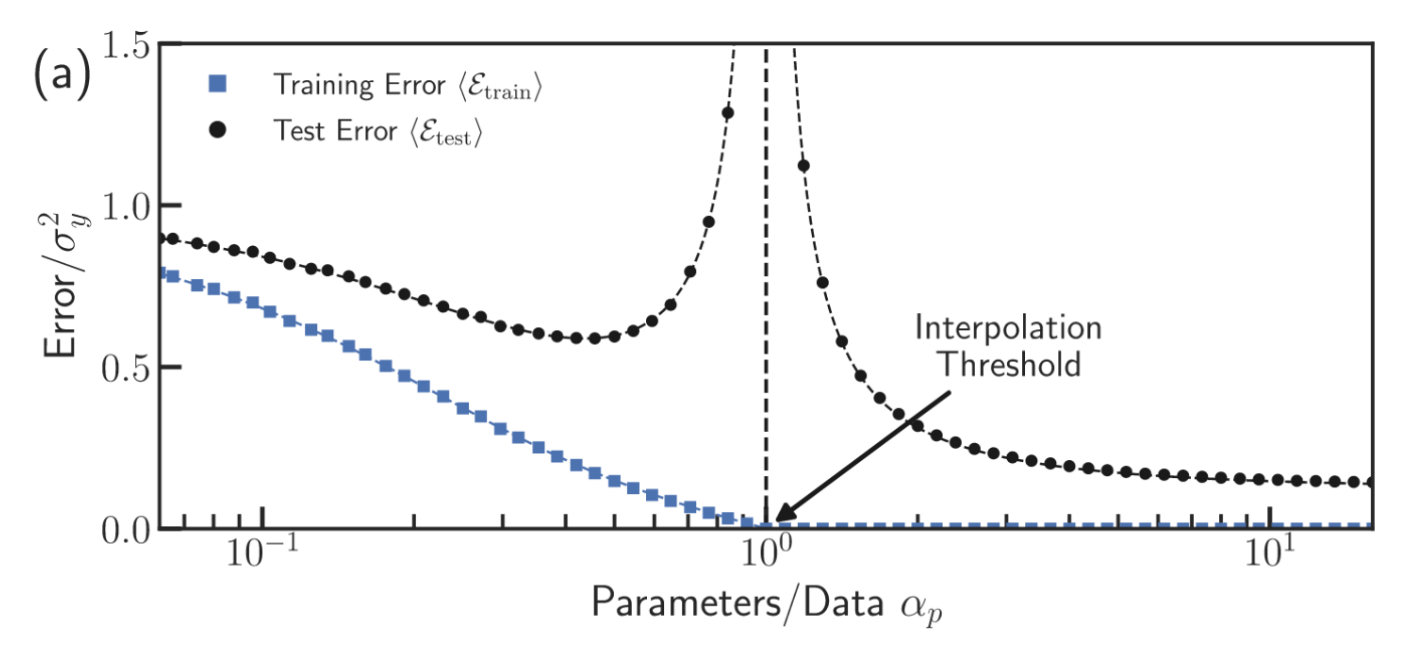
\includegraphics[scale=0.20]{ddd.png}
    \end{center}
    
    \pause

    We choose this optimization problem because \emph{it is the optimization problem that gradient decent implicity minimizes}!
\end{frame}


\begin{frame}{The main equation}

    Unknown to us and the model is the ideal linear parameters $\beta^*$ that truly minimize the test mean squared error. We write 

    $$Y=X\beta^* + E$$

    where $E$ is the uncapturable error. \footnote{$E$ could either be due to a inherently non-linear true relationship or a noisy but linear relationship.}

    \pause

    For the underparameterized regime we have
    \begin{eqnarray*}
        \hat{y}_{test,under} & = & \vec{x}_{test} \cdot (X^T X)^{-1}X^T Y \\
        \hat{y}_{test,under} & = & \vec{x}_{test} (X^T X)^{-1} X^T E  + y^*_{test} \\
        \hat{y}_{test,under} - y^*_{test} & = & \vec{x}_{test} (X^T X)^{-1} X^T E.
    \end{eqnarray*}

\end{frame}

\begin{frame}{The main equation}
    One last step before the main equation...

    \hspace{5cm}
    \pause

    We replace $X$ with its singular value decomposition

    $$X = U \Sigma V^T$$

    with singular values $\sigma_1 > \sigma_2 \dots > \sigma_R > 0.$ The singular values are the square roots of the eigen values of $X$ , ie $\sigma_r=\sqrt{\lambda_r}.$
\end{frame}

\begin{frame}{The main equation}
    We get the following

    \begin{eqnarray*}
        \hat{y}_{test,over} - y^*_{test} = & \sum_{r=1}^R \frac{1}{\sigma_r}(\vec{x}_{test} \cdot \vec{v}_r)(\vec{u}_r \cdot E) & + \text{ bias term}\\
        \hat{y}_{test,under}- y^*_{test} = & \sum_{r=1}^R \frac{1}{\sigma_r}(\vec{x}_{test} \cdot \vec{v}_r)(\vec{u}_r \cdot E) &
    \end{eqnarray*}

    where the bias term is $\vec{x}_{test} (X^T (XX^T)^{-1}X-I_D)\beta^*$.

    \hfill
    \pause

    The variance term causes double descent!

\end{frame}

\begin{frame}{Intuition for components of variance term}
    \begin{equation}
        \sum_{r=1}^R \frac{1}{\sigma_r}(\vec{x}_{test} \cdot \vec{v}_r)(\vec{u}_r \cdot E)
    \end{equation}
    
    Double descent happens when all three of these terms grow large!
    
    \begin{itemize}
        \item How much the \emph{training features} $X$ vary in each direction
            $$\frac{1}{\sigma_r}$$
        \pause
        \item How much, and which direction, the \emph{test features} $\vec{x}_{test}$ vary relative to the \emph{training features} $X$
        $$\vec{x}_{test} \cdot \vec{v}_r$$
        \pause
        \item How well the \emph{best possible model} can correlate the variance in the \emph{training features} $X$ with the \emph{training regression targets} $Y$
            $$\vec{u}_r \cdot E$$
    \end{itemize}

\end{frame}

\begin{frame}{Why do small singular values $\sigma_r$ happen near $P=D$?}
    \begin{center}
        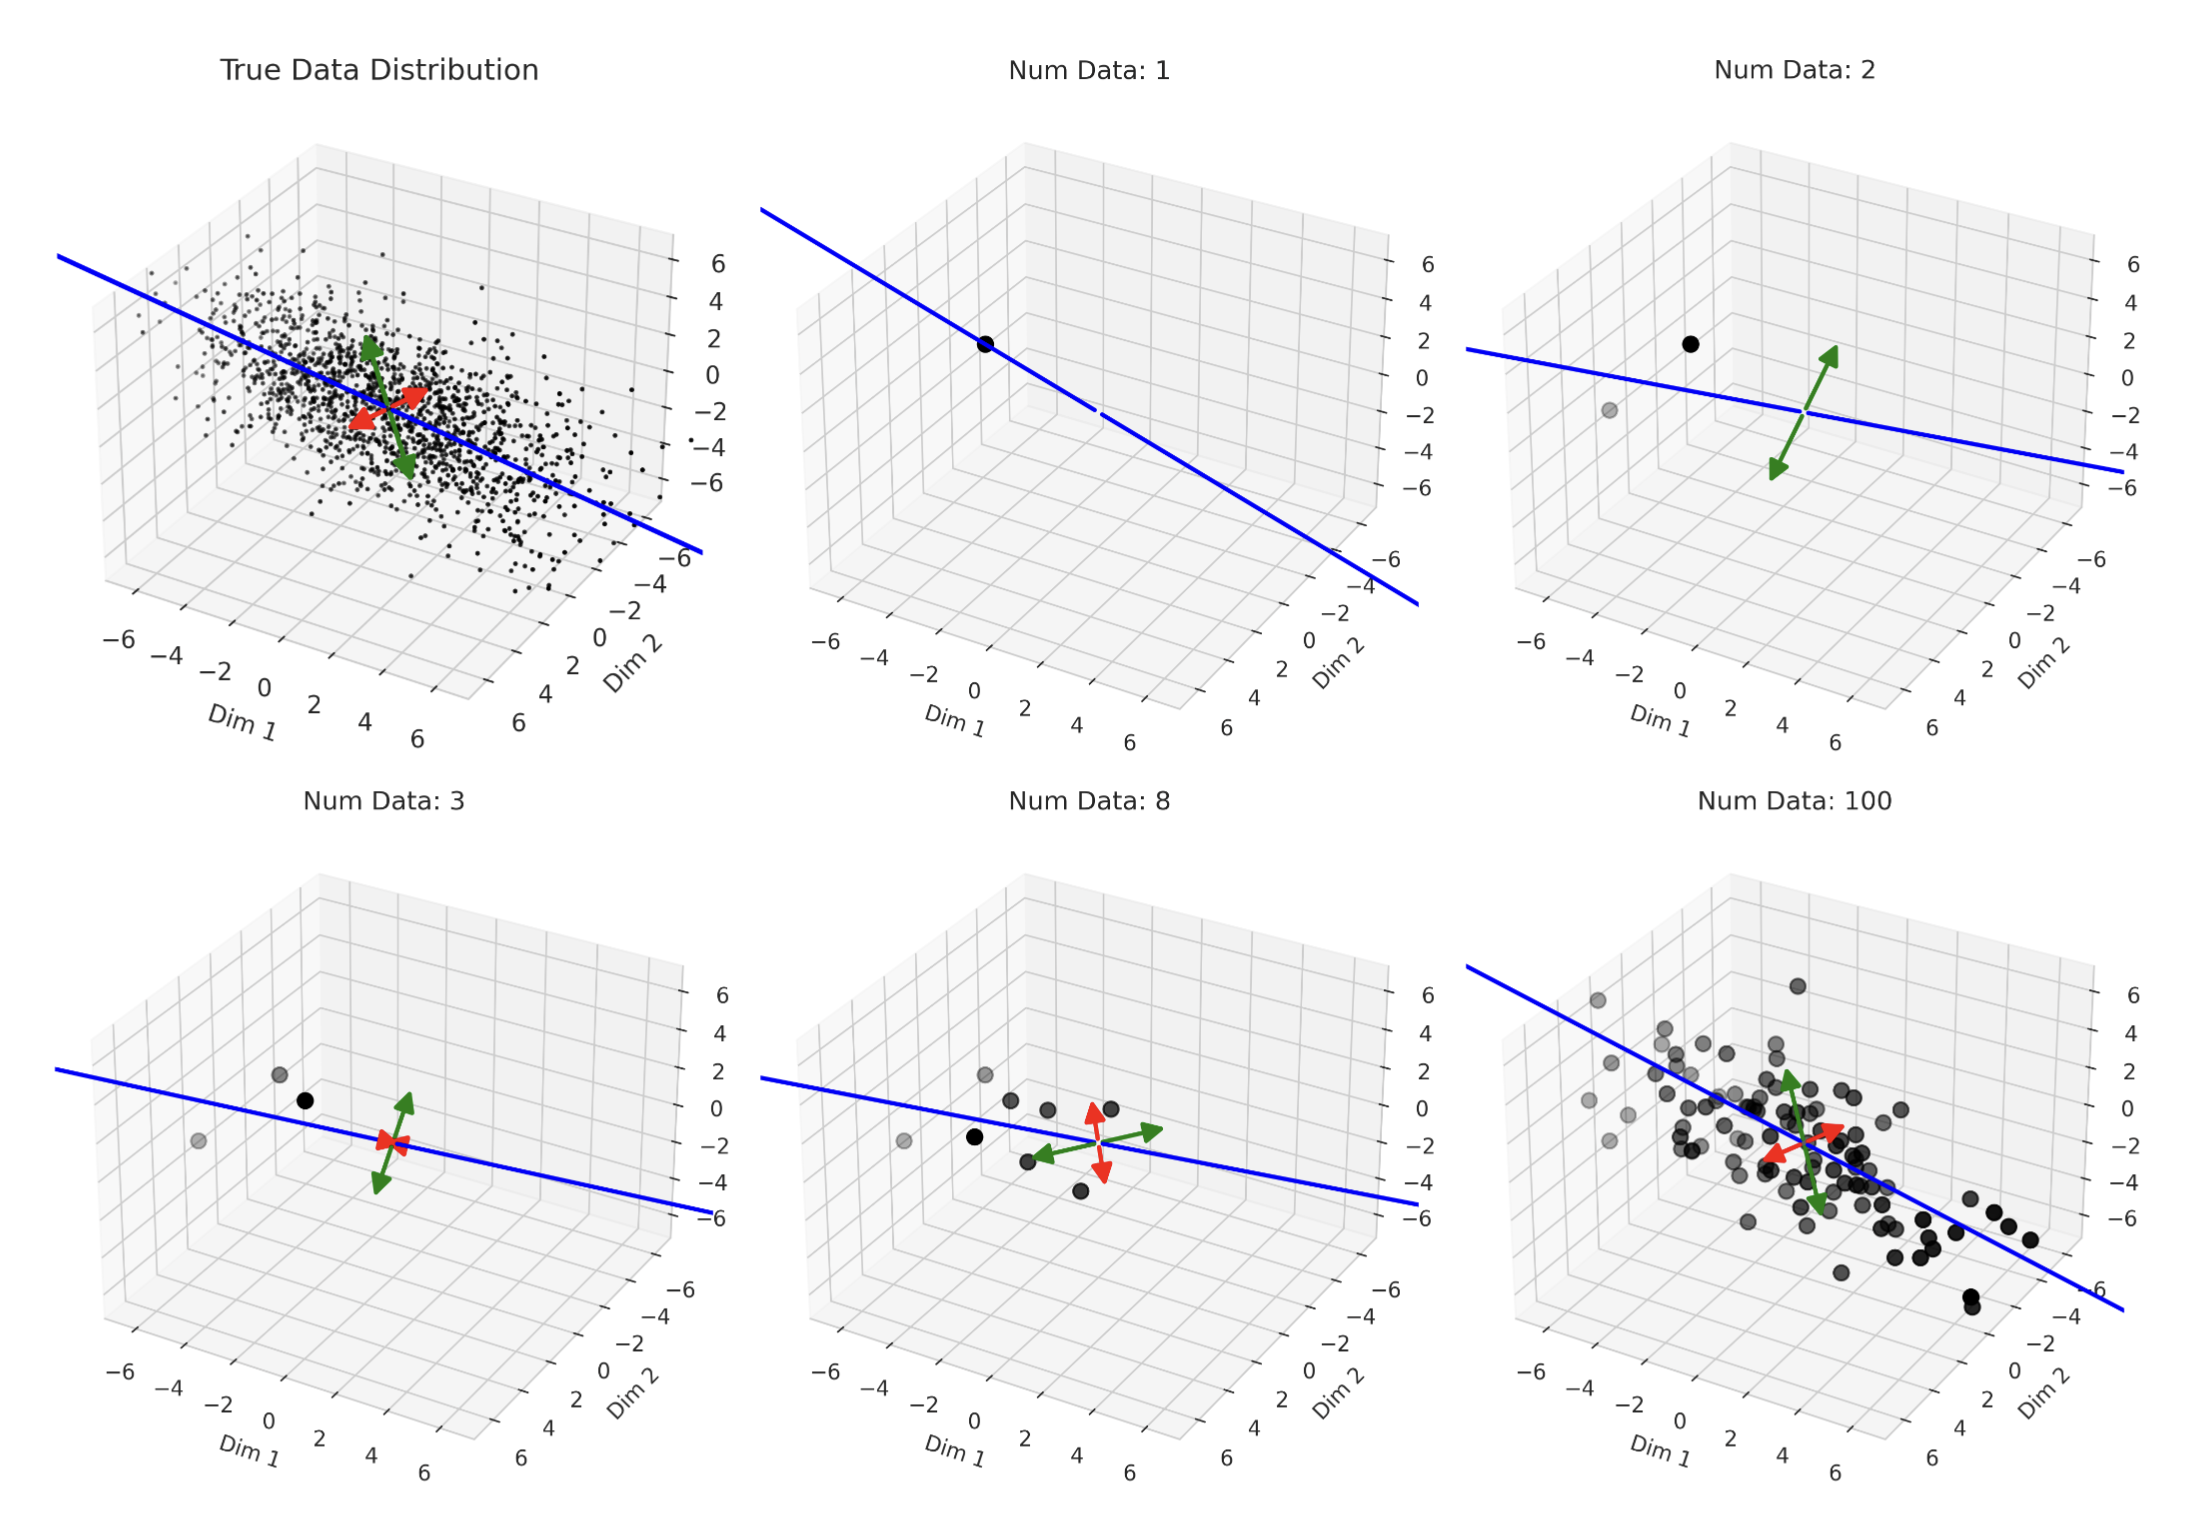
\includegraphics[scale=0.28]{singularvals.png}
    \end{center}
\end{frame}


\begin{frame}{The other components of the variance term}
    \begin{equation*}
        \sum_{r=1}^R \frac{1}{\sigma_r}(\vec{x}_{test} \cdot \vec{v}_r)(\vec{u}_r \cdot E)
    \end{equation*}

    How do the other terms contribute to double descent?

    \begin{itemize}
        \item The test datum does not vary in different directions than the training features. If the test datum lies entirely in the subspace of just a few of the leading singular directions, then double descent is unlikely to occur.
        \item If $E = \vec{0}$, (ie the true function is linear), the variance at and after the interpolation threshold is $0$. 
    \end{itemize}

    \hspace{5cm}
    \pause

    We are going to "remove" each of these contributions to the variance and exhibit that double descent does not occur. 
\end{frame}


\begin{frame}{}
    \begin{center}
        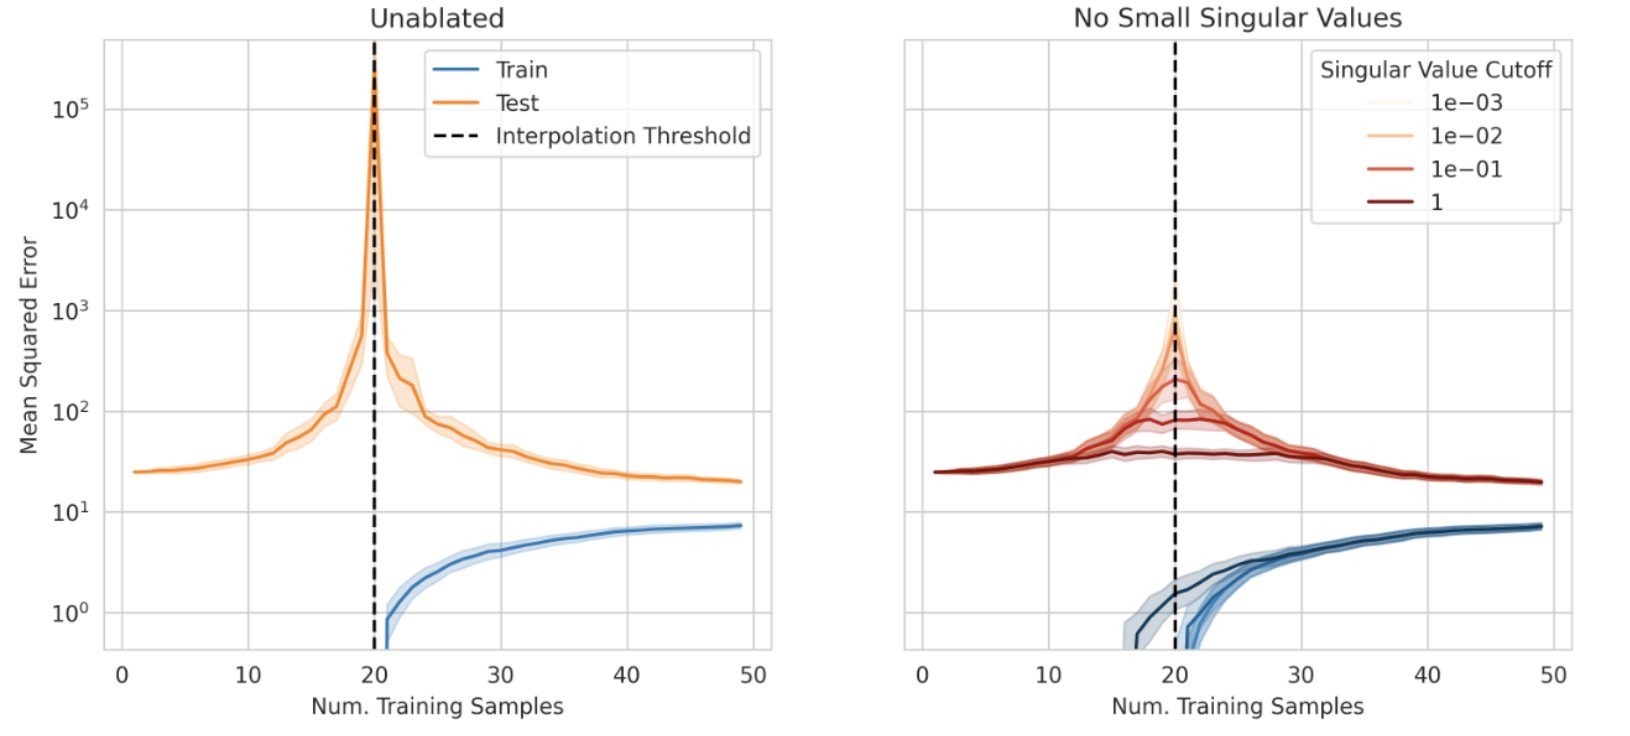
\includegraphics[scale=0.31]{ablate1.png}
        % \hspace{10cm}
        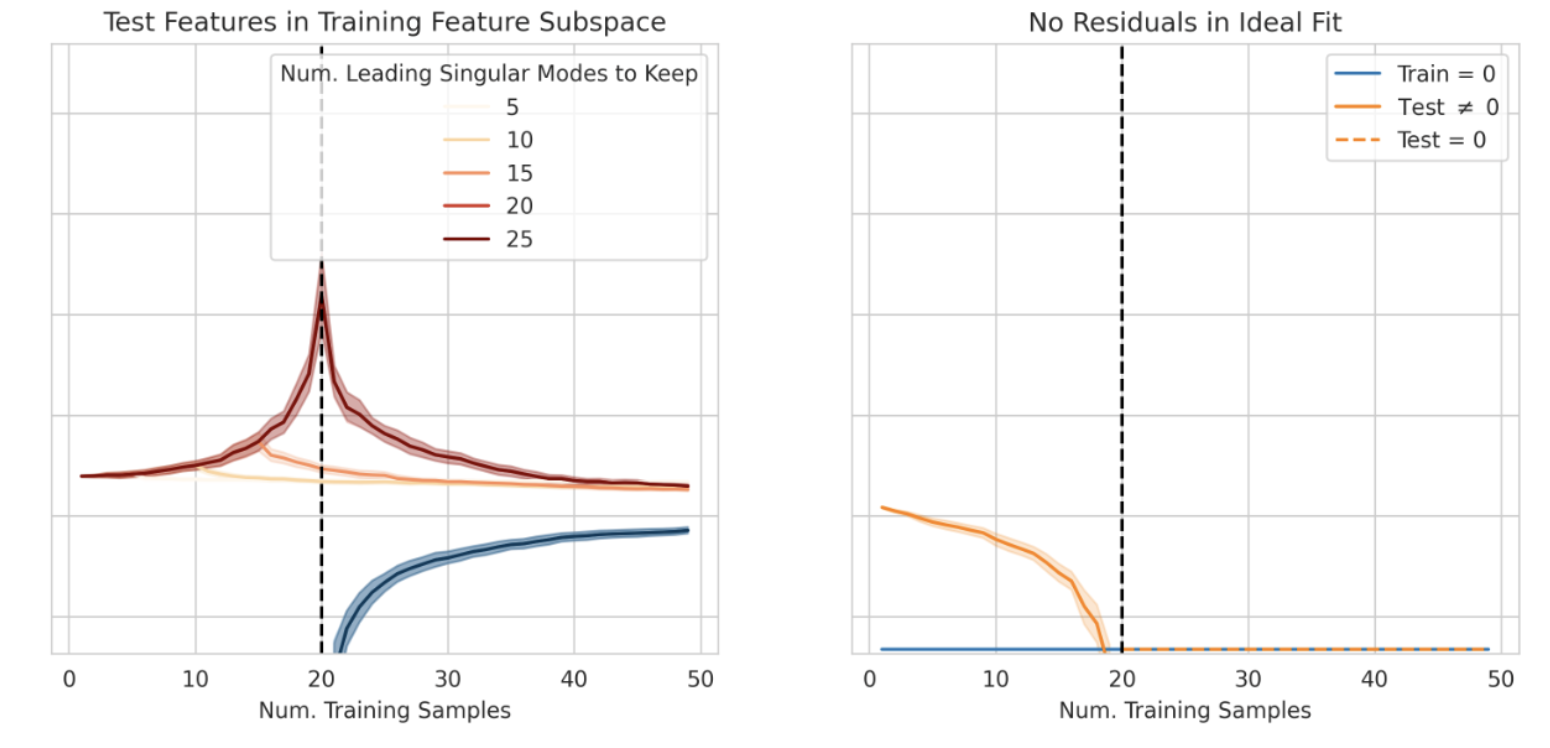
\includegraphics[scale=0.31]{ablate2.png}
    \end{center}
\end{frame}


\begin{frame}{Double descent in nonlinear models - Intuition}

    Neural networks are composed of multiple successive linear regression problems with non-linear activation functions. In many cases training neural networks is equivalent to linear regression on a certain set of features that are functions of the training data. 

    \hspace{5cm}

    \pause
    
    \tiny
    
    "It's interesting to note that we're observing double-descent in the absence of label noise. That is to say: the inputs and targets are exactly the same. Here, the “noise” arises from the lossy compression happening in the down projection.” Our tutorial clarifies that noise in the sense of a random unpredictable quantity is not necessary to produce double descent. Rather, what is necessary is residual errors from the perspective of the model class. Those residual errors could be entirely deterministic, such as a nonlinear model attempting to fit a noiseless linear relationship."
    
    \hspace{5cm}

    Tom Henighan, Shan Carter, Tristan Hume, Nelson Elhage, Robert Lasenby, Stanislav Fort,
    Nicholas Schiefer, and Christopher Olah. Double descent in the condition number. \emph{Transformer
    Circuits Thread, 2023}.
\end{frame}


\begin{frame}{Summary}
    In this talk we covered
    \begin{itemize}
        \item We \emph{identified} double descent in various regression problems
        \item We \emph{interpreted} the components of the variance term in the test error that contribute to double descent
        \item We \emph{ablated} the components for a dataset to demonstrate that double descent occurs only when all components are large near the interpolation threshhold
    \end{itemize}

    \hspace{5cm}

    We also argued that in linear and non-linear models we expect the double descent behavior in a probabalistic sense without intentional ablation.

\end{frame}


\begin{frame}{Thank you for listening!}
    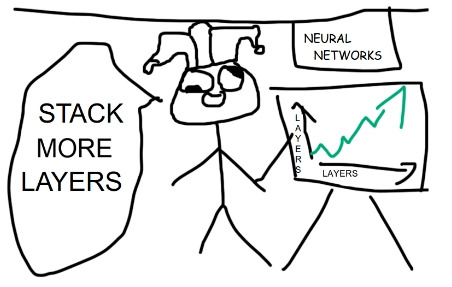
\includegraphics[width=\textwidth]{stackmorelayers.jpg}
\end{frame}


\end{document}